%---------------------------------------------------------------------------
% Chapter 2 - Technology background.
%
%---------------------------------------------------------------------------

\chapter{Technology background}
\label{cha:background}

\chabstract{
Software engineering, unlike any other technical discipline requires deep analysis of the problem domain, prior to starting any new work. Creation of new systems requires to analyze the work of other teams for many reasons, including learning from their mistakes, looking for a bright ideas that fit into a given project or just for an inspiration. This chapter focuses solely on researching the problem domain. Firstly, I would like to describe some projects related to the systems measurement, mostly in distributed processing environments an measurement standards. Later on, I am trying to discuss other projects with a similar functionality. The end of this chapter focuses solely on the semantic aspect of Thesis, the reader may find there a rough description of what is this \lq\lq{}semantic\rq\rq{} thing, as well as a description of technologies that were created to constitute this term.
}

%--------------------------------------------------------------------------- 
% Chapter 2 - Related technologies %

%--------------------------------------------------------------------------- 
\section{Related technologies} 
%---------------------------------------------------------------------------

\subsection{K-WfGrid facilities}

\label{ssec:kwfgrid}

K-WfGrid, which stands for Knowledge-based Workflow System for Grid Applications (\cite{KWfGrid1, flow-cgw04, wct-kwf-book-07}), is both middleware solution that aims in setting up infrastructure for the future Grid environments and consortium of institutions participating in development of this solution. To solve problems caused by dynamic and complex nature of Grid environments, the consortium adopts approaches envisioned by Semantic Web, agent technologies and Grid communities. As an outcome, K-Wf Grid system assists users in the creation of Grid workflows using rule-based expert system. The system adopts ontological descriptions of the environment and applications.

The implemented system, is capable of handling the whole life cycle of workflow, which includes:

\begin{itemize}

\item{semi-automatic composition of application workflow} \item{execution of composed workflow} \item{monitoring performance of execution} \item{analyzing monitoring results} \item{capturing the knowledge contained in this information and tries to {\bf reuse} it in order to construct more efficient, future workflows} \end{itemize}

The main workflow composition functionality is defined as a transformation of a user request document into a solution workflow document in the same data format. The input document must be written using fixed notation - \emph{GWorkflowDL} and may contain some parts of workflow already specified. Parts that are still undefined (called \emph{Unsatisfied Dependency}) contain specification of data that are required at a certain stage of processing. System must find suitable providers of those data in order to generate the whole workflow. Providers, in the form of one or more Grid services are looked up in ontological registry. The workflow is considered to be done, when all unsatisfied dependencies are resolved.

%---------------------------------------------------------------------------

\subsection{OMIS}

\label{ssec:omis}

OMIS, On-Line Monitoring Interface Specification, is another example of efforts aiming at standardization and interoperability between grid monitoring tools. Work on this project was started in 1995. As an outcome, an interface specification in three versions was created: OMIS 1.0\cite{OMIS1}, 2.0\cite{OMIS2} and 2.1.

The main purpose of this project is to define an interface that will allow communication between development tools (e.g. debuggers, performance analyzers or load balancers) and parallel programs running in distributed environment. The researchers had three main goals to achieve: to define an interface that will be extensive and complete to allow usage in existing tools, to allow extendibility and usage in tools not known yet and finally to allow high adaptability to current and future programming paradigms (shared memory, remote procedure call or client/server).

Authors introduced two sub-interfaces to achieve those goals. The first one is for communication between tool and program (monitor/program-interface). The second one lies between tool and monitors (tool/monitor-interface) and has additional extension points. The illustration of this model can be found in Figure~\ref{fig:omis}.

\begin{figure}[ht]

\centering

\includegraphics[width=0.6\textwidth]{omis} \caption{OMIS System Model} \label{fig:omis}

\end{figure}

The OMIS standard defines two kinds of monitoring request - unconditional and conditional ones. Unconditional services specify a set of actions to be performed immediately. It can be interpreted as querying a monitoring mode, where results are obtained instantly and unconditionally. Requests of this type are composed just of one and more information or manipulation services. It creates a request/response communication model. In the second mode, requests contain an event service and a set of actions. In this mode, request tells the monitoring system to execute actions substantially. It creates a publish/subscribe communication model.

\subsection{GMA}

\label{ssec:gma}

GMA stands for Grid Monitoring Architecture~\cite{GMA1,GMA2}. It was originally introduced by Global Grid Forum in 2002. A need to create a shared interface for monitoring grid resources emerged, when several groups of researchers started working on systems facilitating grid monitoring and decided that those tools should be interoperable. The standard is composed of three, high level, types of components. Figure~\ref{fig:gma} depicts them and their relationships.

\begin{figure}[ht]

\centering

\includegraphics[width=0.6\textwidth]{gma} \caption{GMA Components} \label{fig:gma}

\end{figure}

GMA-compatible systems should operate on data that are time stamped performance events. Those events are typed collections of structured data. Measurement data flow always in one direction - from a producer to consumer. Additionally, directory service acts as mediator between them and its work is finished directly after successful establishment of communication link. GMA supports two data exchange models - publish/subscribe (similar to CORBA Event Service) and query/response. What is worth noting, communication may be initiated by both component types - either by a producer or a subscriber.
%--------------------------------------------------------------------------- % Chapter 2 - Similar technologies %

%--------------------------------------------------------------------------- 
\section{Overview of similar monitoring systems} \label{sec:ch2_similar}

%---------------------------------------------------------------------------

\subsection{perfSonar}

The perfSONAR (\cite{perfSonar1,perfSonar2,perfSonar3}) is an infrastructure for network performance monitoring. It aims at making the process of solving end-to-end performance problems on paths crossing several networks easier. It is composed of a set of services delivering performance measurements in a federated environment. This approach allows to characterize the project as a middle ware service that is used by performance measuring tools and diagnostic or visualization applications. The perfSonar layer tries to generate and exchange measurement data between networks. It performs communication using well defined protocols. The architecture of perfSONAR is service oriented, which means that the set of elementary functions (\emph{services}) has been isolated and can be provided by several, independent entities.

The work done on perfSONAR is made around three contexts. First, there is a consortium of organizations that build a network of performance middle ware that is interoperable across multiple networks and useful for a variety of network analysis. The second context is a protocol. It is built on an assumption of fixed, well defined roles (service types) and defines a communication model between components implementing each role. The defined protocol is one of the most important means to achieve interoperability. What is also worth mentioning, the proposed protocol is based on SOAP XML messages format and follows Network Measurement Working Group\footnote{\url{http://nmwg.internet2.edu}} schema. The third context is a set of the implemented software packages that provide the services mentioned above.

The framework defines the following types of services:

\begin{itemize}

\item{ {\bf Measurement Point Service} acts as a service provider. The standard does not define whether it gathers measurement values dynamically, by querying measured components or retrieves static, archived data. It defines only the role of this component as a source of measurement values.}

\item{ {\bf Measurement Archive Service} is responsible for archiving data. It can use any storage facility underneath (Round Robin Database or any other RDBMS). Additionally, it can publish received information. }

\item{ {\bf Lookup Service} enables services to discover each other. It acts as a service-directory, where providers can advertise themselves and requesters are able to find any service needed.}

\item{ {\bf Authentication Service} helps domains which would like to restrict access to given service capabilities for some groups of users. It is responsible for both authorization and authentication. It acts as, so called, an attribute authority which decides which attribute can be disclosed to a resource.}

\item{ {\bf Transformation Service} is a generic service type that allows to create data conversion pipelines. It can perform any function upon data taken from a producer and return transformed data to a consumer.}

\item{ {\bf Topology Service}, provides the framework information about a network topology, which allows, for example, visualization of network maps. Additionally it provides information on geolocation, like GPS coordinates.}

\item{ {\bf Resource Protector Service} - it is used to arbitrate the consumption of limited, shared resources, e.g. network bandwidth.} \end{itemize}

%---------------------------------------------------------------------------

\subsection{SCALEA and SCALEA-G}

SCALEA~\cite{SCALEA1} is a tool for instrumentation, measurement, analysis and visualization of parallel programs execution. It can work with OpenMP, MPI, HPF, and mixed parallel/distributed systems. Its measurements are based on a variety of performance metrics, but SCALEA also supports multiple experiment performance analysis that allows to compare and to evaluate the performance outcome of several experiments.

The architecture of the system distinguishes three main components: SCALEA Instrumentation System (\emph{SIS}), SCALEA Runtime System (\emph{SRS}) and SCALEA Performance Analysis \& Visualization System. SIS can instrument any of FORTRAN, OpenMP, MPI, HPF or even hybrid programs like OpenMP/MPI and allows the user to select code regions and performance metrics of interest. Using this input, SIS inserts probes in the code which will collect all relevant performance information. Those data are saved in a set of profile (trace) files during program execution, which is monitored by SRS. Additionally, the SIS component is responsible for generation of instrumentation description file that can be used to associate gathered performance data back to the input program. Performance Analysis \& Visualization sub system can use raw data gathered either during the program execution or post-mortem.

The main purpose of SCALEA-G (\cite{SCALEA2, SCALEA3}) is to bring the functionality of SCALEA to the grid environment. Originally it was implemented as a set of OGSA services based on Globus Toolkit 3.0, but it was ported then into WSRF-based services with Globus Toolkit 4.0. The most recent implementation of SCALEA-G is composed of the following services:

\begin{itemize}

\item{ {\bf Registry Service}}

\item{ {\bf Directory Service}}

\item{ {\bf Sensor Manager Service} - monitors and measures performance of Grid services. Internally, it is implemented as a WSRF-based service that collects monitoring data from sensors. It supports 2 communication modes - both query/request and subscribe/notify. Collected data are stored in XML containers, based on DBXML.}

\item{ {\bf Dynamic Instrumentation Service}, used for instrumentation of native applications. It uses internally C++ gSOAP+, GSI-plugin and Dyninst.}

\item{ {\bf XML data schema Service}}

\item{ {\bf Client Service}}

\item{ {\bf GUI Component}}

\item{ {\bf Set of Java APIs}}

\end{itemize}

%---------------------------------------------------------------------------

\subsection{DIPAS}

DIPAS~\cite{DIPAS}, which stands for Distributed Performance Analysis Service, is a monitoring platform designed to work with K-WfGrid (see section~\ref{ssec:kwfgrid}). The aim of this project is to provide on-line information about the performance of Grid workflows as well as Grid resources involved in the execution process. These data are used not only by the user, but also by the K-WfGrid middle ware and services, they are a source of knowledge about the performance, which improves the process of semi-automatic workflow construction.

DIPAS provides performance analysis and interpretation for workflows which is based on a novel classification of performance overheads. It allows the user to define the performance constraints. Later, using this input, DIPAS informs the user and client about potential performance problems by interpreting metrics at runtime. Performance analysis of workflows is integrated with tools built-in to the Grid infrastructure, creating a coherent framework.

Additionally, DIPAS provides a web portal for the user to conduct performance monitoring and analysis of workflows with underlying infrastructure. This component substantially simplifies the way that the user interacts with the tool.

The overall architecture of the system is outlined in Figure~\ref{fig:dipas}.

\begin{figure}[ht]
\centering
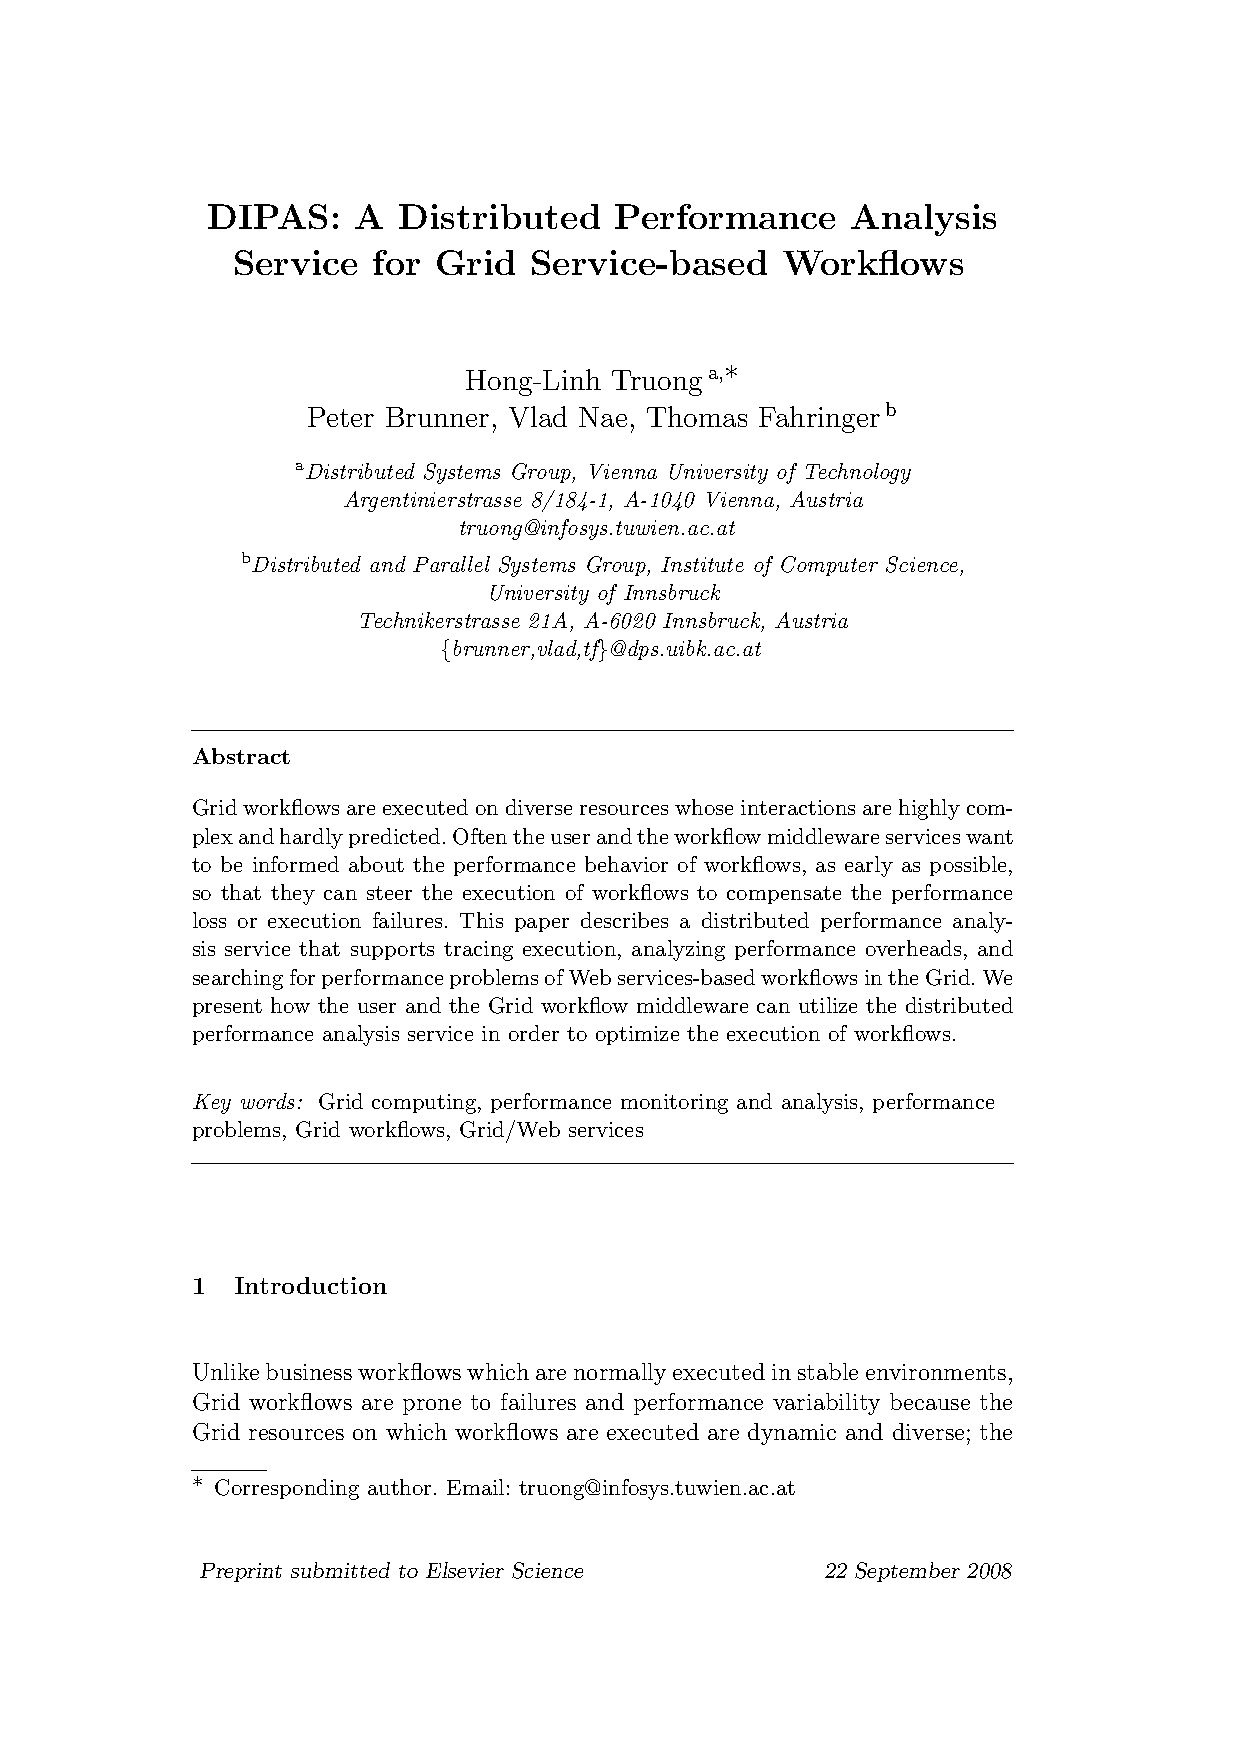
\includegraphics[width=0.6\textwidth]{dipas} 
\caption{Overall architecture of DIPAS} 
\label{fig:dipas}
\end{figure}

%---------------------------------------------------------------------------

\subsection{OCM Family}

As part of work on OMIS (See Section~\ref{ssec:omis}), several tools that are compliant with this interface were introduced. This tool set includes OCM\footnote{\url{http://www.lrr.in.tum.de/Par/tools/Projects/OCM.html}}, OCM-G\footnote{\url{http://grid.cyfronet.pl/ocmg}}, J-OCM\footnote{\url{http://jocm.icsr.agh.edu.pl/sub/main}} and G-PM\footnote{\url{http://gpm.icsr.agh.edu.pl}}.

OCM (\cite{RWspdt98, RW:ppam99b}) - OMIS Compliant Monitoring System is the first tool in the whole set. The main goal of this project was to create a reference implementation of an OMIS compliant monitoring system. Initially it has been supporting PVM (versions 3.3 and 3.4) and then the system was extended to support also the MPI-1.

As a next step in the platform evolution, later on, OCM-G (\cite{axgrid03b}) was introduced. The name of the project is an abbreviation for Grid-enabled OMIS-Compliant Monitoring system. This project focuses on using the OMIS interface with grid environment. It was designed to work with Globus Toolkit and is fully compliant with EGEE environment including gLite 3.x\footnote{\url{http://glite.cern.ch/}} and LCG 2.7.

The latest addition to the set of OMIS-compliant tools is J-OCM - Java oriented monitoring infrastructure (\cite{jocm}). It adds the ability of monitoring JVM based applications. It has extended the OMIS interface by a set of new services, specific for Java, like garbage collection, threads execution, class loading or method invocation. Then the project implementation was focused on monitoring Java Web Services and component oriented applications.

A general architecture shared by all the above implementations is depicted in Figure~\ref{fig:ocmg}.

\begin{figure}[ht]

\centering

\includegraphics[width=0.8\textwidth]{ocm_arch} \caption{Common OMIS-compliant tools architecture diagram} \label{fig:ocmg}

\end{figure}

%---------------------------------------------------------------------------

\subsection{R-GMA}

R-GMA: Relational Grid Monitoring Architecture~(\cite{RGMA1,RGMA2,RGMA3}) is an implementation of GMA, described in Section~\ref{ssec:gma}. Although it implements GMA interface, it adds two exceptions to the standard. First, anyone supplying or obtaining information from R-GMA does not need to know about the Registry component, as its responsibility is addressed by Consumer and Producer components \lq\lq{}behind the scenes\rq\rq{}. The second exception is that information and the monitoring system appears to the end user, like one large relational database and can be queried as such. It is the source of "R" (Relational) in the project name.

All systems that use R-GMA, share information in a virtual database. Data in this database are organized into tables and are managed with the help of standard SQL constructs (like INSERT INTO... or SELECT FROM). With regard to an internal database structure, there is no such thing as a central repository, which holds the data for each table. Virtual database just contains a list of table definitions (\emph{schema}), a list of data providers (\emph{registry}) and a set of rules for deciding which data provider needs to be used while preparing result for given query. These rules are fixed and encoded into an internal component called \emph{mediator}.

The system provides several ways to access the database. There is provided API, with bindings available in Java, C/C++ and Python. Additionally, users can work with the database using the web interface or command line utility.

\section{Semantic Web}
\label{sec:ch2_semantic_web}

In 2001 Tim Berners-Lee, inventor of the World Wide Web and director of World Wide Web Consortium, in his article published in Scientific American\cite{berneslee:semanticWeb} introduced the term Semantic Web. The original idea behind this concept is to change the way how WWW works, from \lq\lq{}web of documents\rq\rq{} towards \lq\lq{}web of data\rq\rq{}. The new kind of web will allow machines to understand the meaning (\emph{semantic}) of information found on the Web. Such an approach will allow developers to create automated agents that can access Web resources in more intelligent way and thus perform more complex tasks on user\rq{}s behalf.

From practical point of view, semantic web is all about two things. First, there is need to define common formats that allows integration and combination of data provided by different, diverse sources. The second big thing is language that can record how the data relates to real world entities. 

Realization of this idea is currently maintained by Semantic Web Activity\footnote{\url{http://www.w3.org/2001/sw}} organized within W3C boundaries. This activity with set of established working groups, is responsible for defining technology standards that must be employed in order to make the Semantic Web operational. Currently, there are following standards defined: RDF, OWL, SPARQL, RDFa, SKOS, RDFS, GRDDL, POWDER, RIF, SAWSDL. Figure~\ref{fig:sem_web_layers} depicts Semantic Web \lq\lq{}Layer Cake\rq\rq{} - layers of technologies setting up the concept together with layers provided by user to create final product. Semantic Web responsibility is all above XML (or URI/IRI) and below Unifying Logic components.

\begin{figure}[ht]
  \centering
  \includegraphics[width=0.6\textwidth]{sem_web_layers}
  \caption{Semantic Web Layer Cake}
  \label{fig:sem_web_layers}
\end{figure}

The following subsections tries to describe roughly most important (in context of this work) of those standards.

\subsection{RDF}

RDF stands for Resource Description Framework (\cite{rdfPrimer:2004}) and is standard model for data interchange on the Web. The main idea behind RDF is to make statements about resources. RDF extends the linking structure of the WWW, by adding usage of URIs to name the relationship between entities together with two ends of the link, creating so called \emph{triples} or subject-predicate-object expressions. In this case, subject denotes the resource, predicates demotes traits or aspects of the resource and expresses a relationship between the subject and the object. Using this model standard allows mixing, exposition and sharing of structured and semi-structured data.

This linking structure forms a directed, labeled graph, where the edges represent a named link between two resources, represented by the graph nodes. Visualization of such a graph forms easiest possible mental model for RDF and is often used in easy-to-understand visual explanations.

In order to make this a bit clearer, let us consider following example. Let us assume, following statement:

\lq\lq{}There is a person called John, whose full name is John Webber, who is British, whose e-mail address is john@agh.edu.pl and is single\rq\rq{}, 
  
which we would like to represent as RDF graph. Illustration of such a graph can be found in Figure~\ref{fig:sample_rdf}.

\begin{figure}[ht]
  \centering
  \includegraphics[width=0.8\textwidth]{sample_rdf}
  \caption{RDF Graph representation of example statement.}
  \label{fig:sample_rdf}
\end{figure}

Pure RDF is just a concept, as its name states - framework. In order to actually use this concept, form of data serialization was introduced - RDFS, which stands for RDF Schema\cite{rdfRef:2004}. Most popular form of RDF serialization is using XML markup (application/rdf+xml mime type). Figure~\ref{fig:sample_rdf_xml} depicts our example using this notation.

\begin{figure}[ht]
  \centering
  \begin{Verbatim}[commandchars=\\\{\},frame=single,framerule=0.2pt]
\PY{c+cp}{<?xml version="1.0"?>}
\PY{n+nt}{<rdf:RDF} \PY{n+na}{xmlns:rdf=}\PY{l+s}{"http://www.w3.org/1999/02/22-rdf-syntax-ns\PYZsh{}"}
             \PY{n+na}{xmlns:pim=}\PY{l+s}{"http://www.agh.edu.pl/pim\PYZsh{}"}\PY{n+nt}{>}
  \PY{n+nt}{<pim:Person} \PY{n+na}{rdf:about=}\PY{l+s}{"http://www.agh.edu.pl/People\PYZsh{}john"}\PY{n+nt}{>}
    \PY{n+nt}{<pim:fullName}\PY{n+nt}{>}John Webber\PY{n+nt}{</pim:fullName>}
    \PY{n+nt}{<pim:email} \PY{n+na}{rdf:resource=}\PY{l+s}{"mailto:john@agh.edu.pl"}\PY{n+nt}{/>}
    \PY{n+nt}{<pim:nationality}\PY{n+nt}{>}British\PY{n+nt}{</pim:nationality>} 
    \PY{n+nt}{<pim:maritialStatus}\PY{n+nt}{>}Single\PY{n+nt}{</pim:maritialStatus>}
  \PY{n+nt}{</pim:Person>}
\PY{n+nt}{</rdf:RDF>}
\end{Verbatim}

  \caption{RDF XML notation of example statement.}
  \label{fig:sample_rdf_xml}
\end{figure}


\subsection{OWL}

RDF is extremely powerful language due to its general form. Although this feature allows one to describe nearly everything using this technology, it also makes it difficult to employ it in real life applications. To bypass those issues, OWL, which stands for Web Ontology Language was introduced. OWL is a stronger language with greater machine interoperability then RDF. Additionally, it comes with larger vocabulary and stronger syntax then RDF.

OWL as a web standard was originally published in 2004, and with reviews and updates, most recent version of standard (called OWL 2.0) was released in 2009\cite{owlRef:2009, owlPrimer:2009}.

OWL comes with following profiles, namely:

\begin{itemize}
\item{ {\bf OWL Lite}}
\item{ {\bf OWL DL}}
\item{ {\bf OWL Full}}
\item{ {\bf OWL EL} (Defined by 2.0 specification)}
\item{ {\bf OWL QL} (Defined by 2.0 specification)}
\item{ {\bf OWL RE} (Defined by 2.0 specification)}
\end{itemize}

Lite, DL and Full profiles were introduced in 2004 version of specification. Each of those sublanguages is a syntactic extension of its simpler predecessor - every legal OWL Lite ontology is legal OWL DL ontology and every legal OWL DL ontology is also legal OWL Full one. Those relations are asymmetric so their inverse doesn\rq{}t hold. 

OWL Lite was initially designed to create relatively simple tools and allow quick migration from systems employing thesauri and other taxonomies. It supports classification hierarchy and simple constraints, e.g. while it supports cardinality, it only permits values of 0 or 1. In practice most of the constructs available in OWL DL can be created using complex combination of OWL Lite features, thus development of tools is almost as difficult as those using OWL DL. 

OWL DL was named that way due to its correspondence with field of research that forms the formal foundation of OWL - Description Logic. It was designed to provide maximum expressiveness while retaining computational completeness, decidability and the availability of practical reasoning algorithms. 

OWL Full is base on a different semantics from OWL Lite or DL and was designed to preserve some compatibility with RDF Schema. 

Profiles introduced by 2.0 spec aims in offering important advantages in particular application scenarios. Each is defined as a syntactic restriction of the OWL 2 Structural Specification and is more restrictive than OWL DL. Restrictions defined in OWL 2 EL allows definition of polynomial time algorithms for all the standard reasoning tasks. It should be used primarily by applications where very large ontologies are employed, and where expressive power can be traded for performance guarantees. OWL 2 QL enables conjunctive queries to be answered in LogSpace (can be solved using a logarithmic amount of memory) using standard relational database technology. This profiles targets application where relatively lightweight ontologies are used to organize large numbers of individuals and where it is useful or necessary to access the data directly via relational queries (e.g.  SQL). The last subset, OWL 2 RL allows implementation of polynomial time reasoning algorithms using rule-extended database technologies that operates directly on RDF triples. It is mostly suitable for applications where relatively lightweight ontologies are used to organize large numbers of individuals and where it is useful or necessary to operate directly on data in the form of RDF triples.


